\documentclass{article}

\usepackage{amsmath}
\usepackage[margin=1in]{geometry}
\usepackage{enumitem}
\usepackage{siunitx}
\usepackage{tikz}

\usetikzlibrary{automata,arrows}

\renewcommand{\theenumi}{\alph{enumi}}
\renewcommand{\theenumii}{\roman{enumii}}

\begin{document}
\title{Computer Networking -- supervision 4}
\author{James Wood}
\maketitle

\section*{Question 1}
Errors can be too severe to correct, so error correcting codes are not used. Reliability can potentially be provided at any level. A frame is retransmitted if an ACK for it wasn't received before the timeout. This technique generally is known as \textit{ARQ}.

\textit{Stop-and-wait} is the simplest ARQ protocol, which involves resending each frame if there is a timeout before the ACK, and only moving on to the next frame when the ACK is received. All frames must be tagged with a sequence number -- either 0 or 1 -- to make sure that a frame resent after a lost ACK is not confused by the receiver with the next frame it is expecting. Stop-and-wait is very inefficient at using the link's capacity.

\textit{Sliding window} is an improvement on stop-and-wait in which multiple frames are sent at once, and distinct ACKs come from each frame. Typically, an ACK will give the sequence number of the first fame not received. The sender then can send any frame with sequence number in the range $[A..A + n)$, where $A$ is the sequence number in the last ACK received, and $n$ is the length of the window. Potentially, the sending window size can be different to the receiving window size. Particularly, a receiving window size of 1 means that the receiver will not queue out-of-order frames.

Alternatively, \textit{concurrent logical channels} can be used. In this system, stop-and-wait can be used for each frame, but there are no guarantees on the order in which frames arrive, so they can be sent concurrently. This achieves efficient use of the link, but may require the sender and receiver to have arbitrarily large buffers.

\section*{Question 2}
\begin{enumerate}
  \item An error-correcting code to deal with the corruptions that happen on a packet-switched network would probably be too large to improve network performance.
  \item
    \begin{enumerate}
      \item Acknowledgements are sent from the receiver to the sender to verify that the message has been delivered. Timeouts declare that if a message hasn't arrived within a set time, it is lost. Taken together, the sender expects an acknowledgement to come within a set time. If this does not happen, the sender will resend the information, so as to achieve at-least-once message delivery.
      \item
        \begin{itemize}
          \item The received packet may have an error. This is detected using the checksum in the packet's header.
          \item 
        \end{itemize}

        A lost NACK is indistinguishable from a lost ACK, so is treated in the same way. This is generally detected by a timeout, and the packet is resent.
      \item This occurs when the ACK for the first packet is lost. The receiver can ignore the packet, but needs to send an ACK so that the sender does not send more copies of the packet.
      \item The ACK can be bundled with any response data, if these data are produced quickly enough (relative to the ACK timeout). This is useful if the original message was to poll the receiver for some value it has stored.
      \item We want a window's worth of packets to take as long to be transmitted as the first packet followed by its ACK. This gives us the relation $\mathit{window\_size} / \mathit{bandwidth} = \mathit{RTT}$ and specific result \SI{2}{Mb}.
      \item
        \begin{itemize}
          \item Typically, the round-trip time will not be known when a connection is first established. To avoid flow problems and packet loss, we choose a conservative window size. We use exponential averaging to approach a good estimate of the round-trip time.
          \item If we are using AIMD, there will be a large drop in window size whenever a packet is dropped. After this, the window will slowly increase in size.
        \end{itemize}
    \end{enumerate}
  \item
    \begin{enumerate}
      \item The sender receives identical ACKs from packets \#2, \#4, and \#5, so retransmits \#3 as soon as it receives the ACK from \#5. This happens when $t = 25$.
      \item The third duplicate ACK received is the ACK for packet \#7. This means that \#3 is retransmitted at $t = 43$.
      \item (a) does not apply, because the sequence would have started with A1, A2, A3, A5. (b) and (e) don't apply, because A4 and A5 arrived in order. (c) and (d) could apply, and would both explain the duplication of A3.
      \item If packet \#4 were dropped, we would receive \#6 before it, because \#6 was sent as soon as A1 was received, so (a) does not apply. (c) and (d) don't explain A4 and A5 being out of order. (b) and (d) do explain this, and they would be indistinguishable to the sender.
      \item Assuming all else functioned as normal, packet \#4 was clearly dropped. It also appears that either \#3 or A3 was duplicated, as there is no other way to receive A3 twice.
    \end{enumerate}
\end{enumerate}

\section*{Question 3}
 

\section*{Question 4}
A:

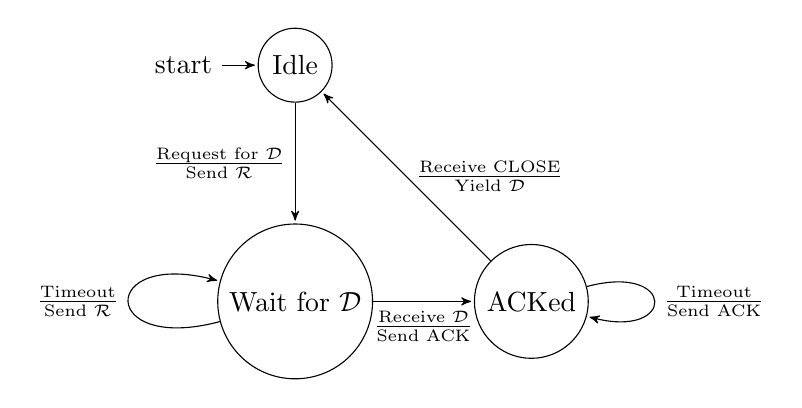
\begin{tikzpicture}[->,>=stealth',shorten >=1pt,auto,node distance=3cm]
  \node[initial,state] (I) {Idle};
  \node[state] (W) [below of=I] {Wait for $\mathcal D$};
  \node[state] (A) [right of=W] {ACKed};

  \path[every node/.style={font=\sffamily\small}]
  (I) edge node [left] {$\textrm{Request for }\mathcal D \over \textrm{Send }\mathcal R$} (W)
  (W) edge [loop left] node {$\textrm{Timeout} \over \textrm{Send }\mathcal R$} (W)
  (W) edge node [below] {$\textrm{Receive }\mathcal D \over \textrm{Send ACK}$} (A)
  (A) edge [loop right] node {$\textrm{Timeout} \over \textrm{Send ACK}$} (A)
  (A) edge node [right] {$\textrm{Receive CLOSE} \over \textrm{Yield }\mathcal D$} (I)
  ;
\end{tikzpicture}

B:

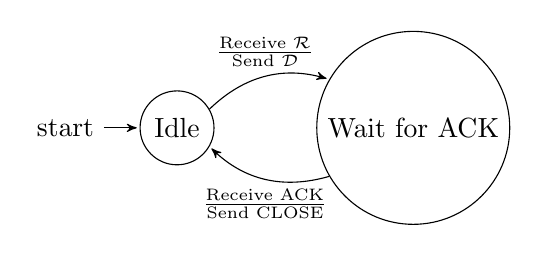
\begin{tikzpicture}[->,>=stealth',shorten >=1pt,auto,node distance=3cm]
  \node[initial,state] (I) {Idle};
  \node[state] (W) [right of=I] {Wait for ACK};

  \path[every node/.style={font=\sffamily\small}]
  (I) edge [bend left] node [above] {$\textrm{Receive }\mathcal R \over \textrm{Send }\mathcal D$} (W)
  (W) edge [bend left] node [below] {$\textrm{Receive ACK} \over \textrm{Send CLOSE}$} (I)
  ;
\end{tikzpicture}

\section*{Question 5}
\begin{enumerate}
  \item
    \begin{enumerate}
      \item A \SI{3000}{B} TCP segment carries \SI{2960}{B} ($3000 - 20 - 20$) of data. A fragment of size \SI{1500}{B} carries \SI{1460}{B} of data. Because ${2960 \over 1460} \in (2,3]$, three fragments of each original packet are required on the link between the routers. Routers re\"assemble fragmented packets when receiving, so \SI{3000}{B} packets are delivered to $H_B$.

        A better choice of TCP segment size would have been \SI[parse-numbers=false]{(1460 * 2 + 20 + 20)}{B} (which is \SI{2960}{B}), or simply \SI{1500}{B}. This would reduce the number of packets on the network, which would help with flow control at the routers. It would also mean that there is a better data-to-header ratio, but headers for these packets are relatively small anyway.
      \item IPv6 has no facilities for fragmentation, so the hosts would have had to ascertain the \SI{1500}{B} MTU of the network, then sent packages of that size.
    \end{enumerate}
  \item
    \begin{enumerate}
      \item $M$ is the time between the sending of a packet and the reception of the corresponding ACK. This measurement is only taken for packets that have not been retransmitted at all, so as to avoid ambiguity in the send time.
      \item $R$ is a weighted average of all collected $M$ values, biased exponentially towards more recent values. $D$ represents the uncertainty in the RTT estimate $R$. If $M$ is closer to $R$ than estimated by $D$, $D$ will decrease, and the reverse for $M$ far from $R$. Similarly to $R$, this is weighted so as to not be affected by large transient changes in $\lvert M - R \rvert$. The formula for $\mathcal R$ is chosen to allow for the mean RTT plus 4 times the expected uncertainty before declaring a packet lost.

        The specific values of 0.25 and 0.875 are chosen because they have particularly simple binary representations ($0.01_2$ and $0.111_2$, respectively). Multiplication by $h$ is a simple bit shift, and $\alpha \cdot R$ can be computed as $R - 0.001_2 \cdot R$, which again just requires a bit shift and an addition. Taken together, these mean that general multiplication is not required, and the formulae can be programmed in hardware relatively simply.
    \end{enumerate}
\end{enumerate}

\end{document}
